\documentclass[14pt]{extarticle}
%\documentclass[a4paper]{extarticle}
%\documentclass[12pt, a4paper]{article}

% === Кодировки и язык ===
\usepackage[T2A]{fontenc}          % Кириллическая кодировка шрифтов
\usepackage[utf8]{inputenc}        % Кодировка исходного файла - UTF-8
\usepackage[russian]{babel}        % Поддержка русского языка

% === Основные пакеты ===
\usepackage{graphicx}              % Работа с изображениями
\usepackage{amsmath}               % Математические формулы
\usepackage{indentfirst}           % Отступ в первом абзаце раздела
\usepackage{fancyvrb}              % Расширенный режим Verbatim
\usepackage{fvextra}               % Поддержка breaklines и UTF-8 в Verbatim
\usepackage{comment}               % Блоки комментариев
%\usepackage{enumitem}              % Гибкая настройка списков
%\usepackage[skip=0pt]{parskip}     % Убирает лишние отступы между абзацами
\usepackage{float}
%\usepackage{makecell}

\usepackage{pdflscape}

\usepackage{listings}
% Переименовываем стандартное слово "Listing" в "Листинг"
\renewcommand{\lstlistingname}{Листинг}
\usepackage{amssymb} % Требуется для символа \hookrightarrow
\lstset{
    %basicstyle=\ttfamily,         % Моноширинный шрифт
    numbers=left,                 % Номера строк слева
    numberstyle=\tiny,            % Размер шрифта для номеров строк
    frame=single,                 % Одинарная рамка вокруг кода
    breaklines=true,              % Автоматический перенос длинных строк
    postbreak=\mbox{\tiny\ensuremath{\hookrightarrow}\space},
    %tabsize=4,                    % Размер табуляции
    %showstringspaces=false        % Отключение визуализации пробелов в строках
    }

% === Разметка страницы и вспомогательные пакеты ===
\usepackage{geometry}              % Настройка полей - используется ниже вместо ручных команд

% === Гиперссылки ===
\usepackage{hyperref}

% === Геометрия страницы ===
\geometry{
  % textheight=24cm,
  % textwidth=16cm,
  left=2.5cm,
  top=1cm
}

\begin{document}

\thispagestyle{empty} % Убираем нумерацию первой страницы

\begin{center}
    МИНИСТЕРСТВО НАУКИ И ВЫСШЕГО ОБРАЗОВАНИЯ\\ РОССИЙСКОЙ ФЕДЕРАЦИИ

    Федеральное государственное автономное образовательное учреждение высшего образования «Санкт-Петербургский политехнический университет Петра Великого»

    Институт компьютерных наук и кибербезопасности

    Высшая школа технологий искусственного интеллекта

    Направление: 02.03.01 <<Математика и компьютерные науки>>

    % Основной заголовок
    \vspace{3cm}
    {\Large
        Отчёт о выполнении курсовой работы

        по дисциплине <<Методы проектирования баз данных>>

        на тему <<Нереляционные возможности СУБД PostgreSQL>>


    }
    \vspace{3cm}

    % Блок с исполнителем и проверяющим
    \begin{minipage}{\textwidth}
        Выполнила студентка группы \\
        №5130201/40101 \hfill Старкова Ю.А.

        \vspace{0.5cm}

        Проверил доцент ВШТИИ
        \hfill Попов С.Г.
    \end{minipage}

    % Блок с подписью и датой
    \vspace{1cm}
    \hfill
    <<\line(1,0){1cm}>> \line(1,0){3cm}\, 2026\,г.

    % Город и год
    \vspace{2cm}
    Санкт-Петербург \\
    2026
\end{center}
\newpage
\begin{abstract}

    тут аннотация

\end{abstract}
\newpage

%содержание
\tableofcontents

\newpage


\addcontentsline{toc}{section}{Введение}
\section*{Введение}
тут введение
\newpage


\section{Постановка задачи}
\newpage

\section{Представления}

\subsection{Создание представления}
\textbf{Формулировка задания на русском языке.}

Создать представление, в котором необходимо для каждой коровы
подсчитать количество лактаций и количество рационов,
по которым она питалась.

Команда создания представления на языке SQL приведена в листинге \ref{lst:create_view}.

\begin{lstlisting}[caption={Создание представления}, label={lst:create_view}]
CREATE VIEW Cow_Lactation_Diet_Count AS
SELECT Cow.id_Cow, COUNT(DISTINCT Lactation.id_Lactation) AS lactation_count,
COUNT(DISTINCT Diet.id_Diet) AS diet_count
FROM Cow
LEFT JOIN Lactation ON Lactation.id_Cow = Cow.id_Cow
LEFT JOIN Nutrition ON Nutrition.id_Cow = Cow.id_Cow
LEFT JOIN Feeding_plan ON Feeding_plan.id_Feeding_plan = Nutrition.id_Feeding_plan
LEFT JOIN Diet ON Diet.id_Diet = Feeding_plan.id_Diet
GROUP BY Cow.id_Cow;
\end{lstlisting}

На рисунке \ref{fig:create_view_res} продемонстрирована часть таблицы ---
результат выполнения команды создания представления.
\begin{figure}[H]
    \centering
    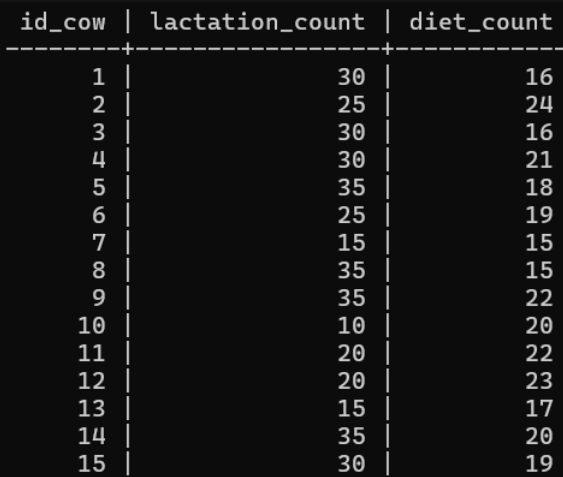
\includegraphics[width=0.5\linewidth]{images/create_view_res.png}
    \caption{Результат выполнения команды создания представления}
    \label{fig:create_view_res}
\end{figure}

На рисунке \ref{fig:create_view_exp}
продемонстрирован план выполнения SQL-запроса, лежащего в основе созданного представления.
\begin{figure}[H]
    \centering
    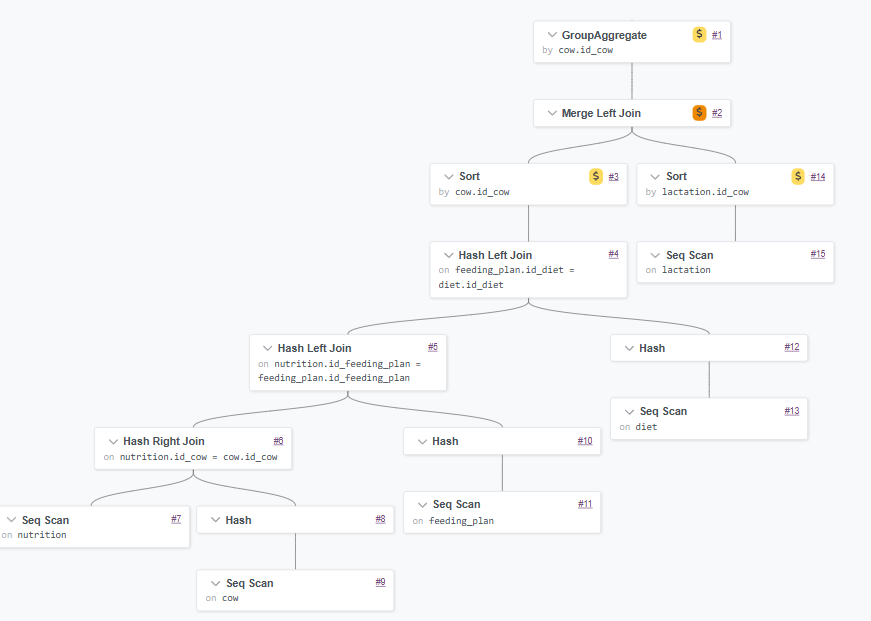
\includegraphics[width=\linewidth]{images/create_view_exp.png}
    \caption{Графическое представление последовательности выполнения запроса при создании представления}
    \label{fig:create_view_exp}
\end{figure}


\textbf{Текстовое объяснение последовательности выполнения запроса, лежащего
в основе создания  представления.}

В запросе сначала осуществляется обращение к базовой таблице \\\texttt{Cow}.
Затем к ней последовательно присоединяются таблицы \texttt{Lactation, Nutrition, Feeding\_plan} и
\texttt{Diet} с использованием оператора левого внешнего соединения (\texttt{LEFT JOIN}).
После объединения данных строки группируются по уникальному идентификатору коровы (\texttt{Cow.id\_Cow})
с помощью \texttt{GROUP BY}. Для каждой группы (каждой коровы) с помощью агрегатной функции
\texttt{COUNT} и ключевого слова \texttt{DISTINCT} вычисляется количество уникальных записей
лактаций и уникальных рационов. Итоговый результат сохраняется в базе данных как виртуальная
таблица (представление) под именем \texttt{Cow\_Lactation\_Diet\_Count}.

\textbf{Реляционная формула команды.}
\[
    \text{Cow\_Lactation\_Diet\_Count} \leftarrow \mathcal{G}_{\substack{
        \text{Cow.id\_Cow}, \\
        \text{COUNT(DISTINCT Lactation.id\_Lactation)} \rightarrow \text{lactation\_count}, \\
        \text{COUNT(DISTINCT Diet.id\_Diet)} \rightarrow \text{diet\_count}
    }} (
\]
\[
    \text{Cow} \overset{\text{LEFT}}{\bowtie}_{\text{Cow.id\_Cow}=\text{Lactation.id\_Cow}} \text{Lactation}
\]
\[
    \overset{\text{LEFT}}{\bowtie}_{\text{Cow.id\_Cow}=\text{Nutrition.id\_Cow}} \text{Nutrition}
\]
\[
    \overset{\text{LEFT}}{\bowtie}_{\text{Nutrition.id\_Feeding\_plan}=\text{Feeding\_plan.id\_Feeding\_plan}} \text{Feeding\_plan}
\]
\[
    \overset{\text{LEFT}}{\bowtie}_{\text{Feeding\_plan.id\_Diet}=\text{Diet.id\_Diet}} \text{Diet}
    )
\]

\subsection{Запрос 1}
\textbf{Формулировка запроса 1 на русском языке.}

Подсчитать количество коров, у которых было больше 2 лактаций.

Код запроса на языке SQL представлен в листинге \ref{lst:запрос_1}.

\begin{lstlisting}[caption={Запрос 1}, label={lst:запрос_1}]
    SELECT COUNT(*) FROM Cow_Lactation_Diet_Count WHERE lactation_count > 2;
\end{lstlisting}

На рисунке \ref{1view_res} продемонстрирован результат выполнения запроса.

\begin{figure}[H]
    \centering
    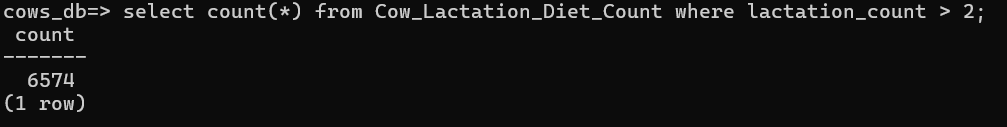
\includegraphics[width=\linewidth]{images/1view_res.png}
    \caption{Результат выполнения запроса 1}
    \label{1view_res}
\end{figure}

На рисунке \ref{1view_exp}
продемонстрировано графическое представление последовательности выполнения запроса 1.
\begin{figure}[H]
    \centering
    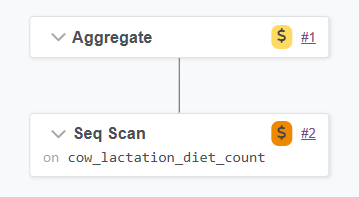
\includegraphics[width=0.6\linewidth]{images/1view_exp.png}
    \caption{Графическое представление последовательности выполнения запроса 1}
    \label{1view_exp}
\end{figure}

\textbf{Текстовое объяснение последовательности выполнения запроса 1.}

В запросе осуществляется обращение к ранее созданному представлению\\
\texttt{Cow\_Lactation\_Diet\_Count}.
Сначала с помощью оператора \texttt{WHERE} отфильтровываются записи,
оставляя только те строки, в которых значение атрибута \texttt{lactation\_count}
(количество лактаций) строго больше двух.
Затем для полученного набора данных применяется агрегатная функция \texttt{COUNT},
которая подсчитывает итоговое количество строк (коров),
удовлетворяющих заданному условию.

\textbf{Реляционная формула запроса.}
\[
    \mathcal{G}_{\text{COUNT(*)} \rightarrow \text{cow\_count}} (
\]
\[
    \sigma_{\text{lactation\_count} > 2} (
    \]
    \[
    \text{Cow\_Lactation\_Diet\_Count}))
\]

\subsection{Запрос 2}

\textbf{Формулировка запроса 2 на русском языке.}

Для каждой коровы вывести возраст, количество лактаций, количество рационов
и кормов по которым она питалась.

Код запроса на языке SQL представлен в листинге \ref{lst:запрос_2}.

\begin{lstlisting}[caption={Запрос 2}, label={lst:запрос_2}]
    SELECT Cow.id_Cow, Cow.Age, Cow_Lactation_Diet_Count.lactation_count,
    Cow_Lactation_Diet_Count.diet_count, COUNT(DISTINCT Feeds.id_Feeds) AS feed_count
    FROM Cow_Lactation_Diet_Count
    JOIN Cow ON Cow.id_Cow = Cow_Lactation_Diet_Count.id_Cow
    LEFT JOIN Nutrition ON Nutrition.id_Cow = Cow.id_Cow
    LEFT JOIN Feeding_plan ON Feeding_plan.id_Feeding_plan = Nutrition.id_Feeding_plan
    LEFT JOIN Feeds ON Feeds.id_feeds = Feeding_plan.id_feeds
    GROUP BY Cow.id_Cow, Cow.Age, Cow_Lactation_Diet_Count.lactation_count, Cow_Lactation_Diet_Count.diet_count;
\end{lstlisting}

На рисунке \ref{2view_res} продемонстрирован результат выполнения запроса \\(часть таблицы).

\begin{figure}[H]
    \centering
    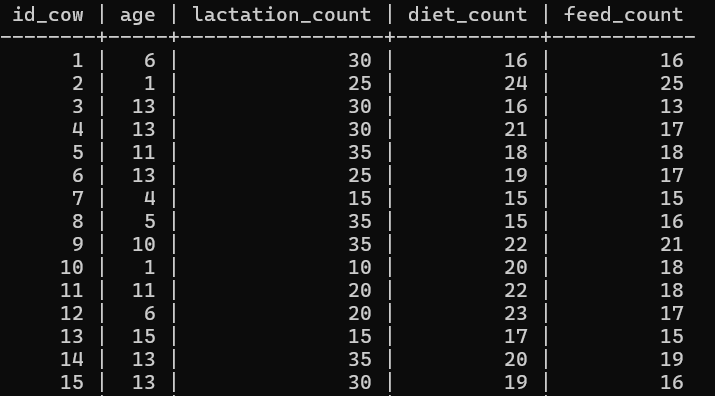
\includegraphics[width=\linewidth]{images/2view_res.png}
    \caption{Результат выполнения запроса 2}
    \label{2view_res}
\end{figure}

На рисунке \ref{2view_exp}
продемонстрировано графическое представление последовательности выполнения запроса 2.
\begin{figure}[H]
    \centering
    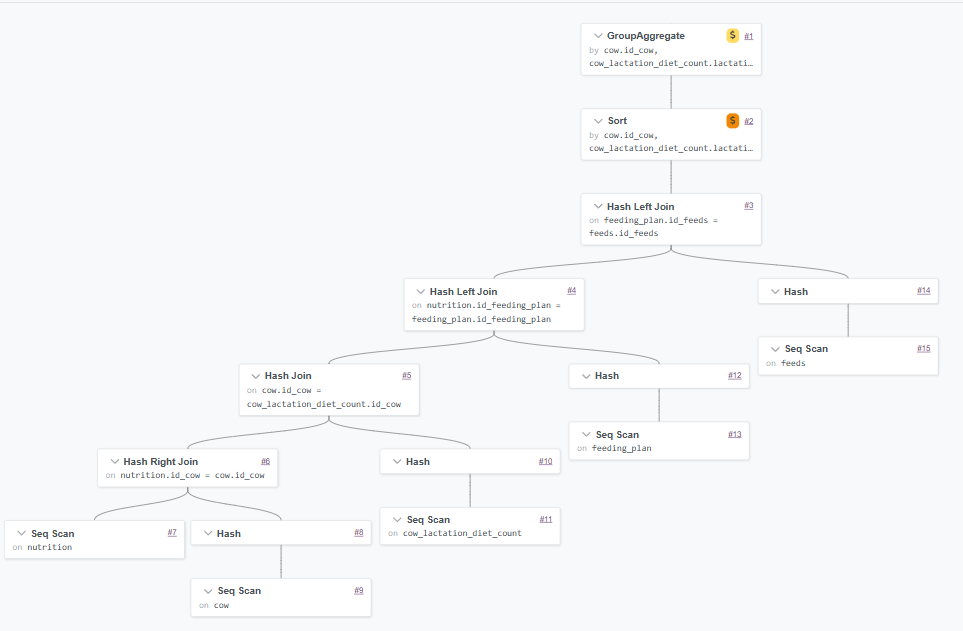
\includegraphics[width=\linewidth]{images/2view__exp.png}
    \caption{Графическое представление последовательности выполнения запроса 2}
    \label{2view_exp}
\end{figure}

\textbf{Текстовое объяснение последовательности выполнения запроса 2.}

В запросе осуществляется обращение к представлению \\\texttt{Cow\_Lactation\_Diet\_Count},
к которому с помощью внутреннего соединения (\texttt{JOIN})
присоединяется базовая таблица \texttt{Cow}.
Затем к полученному результату последовательно присоединяются таблицы
\texttt{Nutrition, Feeding\_plan} и \texttt{Feeds} с использованием оператора
левого внешнего соединения (\texttt{LEFT JOIN}).
После объединения данных строки группируются по идентификатору и возрасту коровы,
а также по количествам лактаций и рационов, полученным из представления.
В завершение для каждой группы с помощью агрегатной функции \texttt{COUNT} и
ключевого слова \texttt{DISTINCT} вычисляется количество уникальных идентификаторов
кормов (\texttt{feed\_count}).

\textbf{Реляционная формула запроса.}
\[
    \mathcal{G}_{\substack{
        \text{Cow.id\_Cow, Cow.Age}, \\
        \text{Cow\_Lactation\_Diet\_Count.lactation\_count}, \\
        \text{Cow\_Lactation\_Diet\_Count.diet\_count}, \\
        \text{COUNT(DISTINCT Feeds.id\_Feeds)} \rightarrow \text{feed\_count}
    }} (
\]

\[
    \text{Cow\_Lactation\_Diet\_Count} \bowtie_{\text{Cow\_Lactation\_Diet\_Count.id\_cow}=\text{Cow.id\_cow}} \text{Cow}
\]
\[
    \overset{\text{LEFT}}{\bowtie}_{\text{Cow.id\_cow}=\text{Nutrition.id\_cow}} \text{Nutrition}
\]
\[
    \overset{\text{LEFT}}{\bowtie}_{\text{Nutrition.id\_Feeding\_plan}=\text{Feeding\_plan.id\_Feeding\_plan}} \text{Feeding\_plan}
\]
\[
    \overset{\text{LEFT}}{\bowtie}_{\text{Feeding\_plan.id\_feeds}=\text{Feeds.id\_feeds}} \text{Feeds})
\]


\newpage
\addcontentsline{toc}{section}{Заключение раздела <<Представления>>}
\section*{Заключение раздела <<Представления>>}

В результате работы было создано представление \\\texttt{Cow\_lactation\_diet\_count},
в котором для каждой коровы подсчитаны количество лактаций и рационов, по которым
она питалась. Были составлены два запроса: первый --- непосредственно к представлению,
второй --- с использованием представления при объединении с другими таблицами.
К каждому запросу составлены реляционные формулы и представлены графические планы
выполнения.
\newpage

\section{Триггеры}
\textbf{Формулировка задания.}

Создать таблицу, в которой с помощью триггеров для каждой коровы
поддерживаются актуальные значения количества лактаций и назначенных рационов питания.

\subsection{Создание таблицы}
\textbf{Текстовое объяснение последовательности выполнения команды создания таблицы.}

При выполнении команды создается физическая таблица \\\texttt{Cow\_lactation\_diet\_count}.
В структуре таблицы определяются три поля целочисленного типа (\texttt{INT}):
первичный ключ \texttt{id\_Cow} для идентификации коровы,
а также столбцы \texttt{Lactation\_count} и \texttt{Diet\_count},
предназначенные для хранения актуальных значений количества лактаций и рационов
каждой коровы.

SQL-код создания таблицы \texttt{Cow\_lactation\_diet\_count} приведен в листинге
\ref{lst:Cow_lactation_diet_count}.

\begin{lstlisting}[caption={Создание таблицы Cow\_lactation\_diet\_count}, label={lst:Cow_lactation_diet_count}]
CREATE TABLE IF NOT EXISTS Cow_lactation_diet_count (
    id_Cow INT PRIMARY KEY,
    Lactation_count INT,
    Diet_count INT
);
\end{lstlisting}

\textbf{Текстовое объяснение последовательности выполнения команды заполнения таблицы.}

Для заполнения таблицы \texttt{Cow\_lactation\_diet\_count}
используется команда \texttt{INSERT INTO} в сочетании с подзапросом, считывающим выборку 
\texttt{SELECT}.
В подзапросе к таблице \texttt{Cow} последовательно присоединяются таблицы
\texttt{Lactation, Nutrition, Feeding\_plan} и \texttt{Diet} с помощью
левого внешнего соединения (\texttt{LEFT JOIN}).
Данные группируются по ключевому полю \texttt{Cow.id\_Cow},
после чего агрегатная функция \texttt{COUNT} с ключевым словом \texttt{DISTINCT} рассчитывает количество уникальных лактаций и рационов для каждой коровы. Полученные значения вставляются в соответствующие столбцы созданной таблицы.

В листинге \ref{lst:Cow_lactation_diet_count_заполнение}
приведен SQL-код заполнения таблицы \\\texttt{Cow\_lactation\_diet\_count} данными.

\begin{lstlisting}[caption={Заполнение таблицы Cow\_lactation\_diet\_count}, label={lst:Cow_lactation_diet_count_заполнение}]
INSERT INTO Cow_lactation_diet_count (id_Cow, Lactation_count, Diet_count)
SELECT Cow.id_Cow, 
    COUNT(DISTINCT Lactation.id_Lactation), 
    COUNT(DISTINCT Diet.id_Diet)
FROM Cow 
LEFT JOIN Lactation ON Lactation.id_Cow = Cow.id_Cow
LEFT JOIN Nutrition ON Nutrition.id_Cow = Cow.id_Cow
LEFT JOIN Feeding_plan ON Feeding_plan.id_Feeding_plan = Nutrition.id_Feeding_plan
LEFT JOIN Diet ON Diet.id_Diet = Feeding_plan.id_Diet
GROUP BY Cow.id_Cow;
\end{lstlisting}

На рисунке \ref{fig:схема_бд_англ} представлена схема базы данных на английском языке
с добавлением созданной таблицы \texttt{Cow\_lactation\_diet\_count} и указанием триггеров.

\clearpage
\newgeometry{margin=1cm}
\begin{landscape}
    \begin{figure}[p]
        \centering
        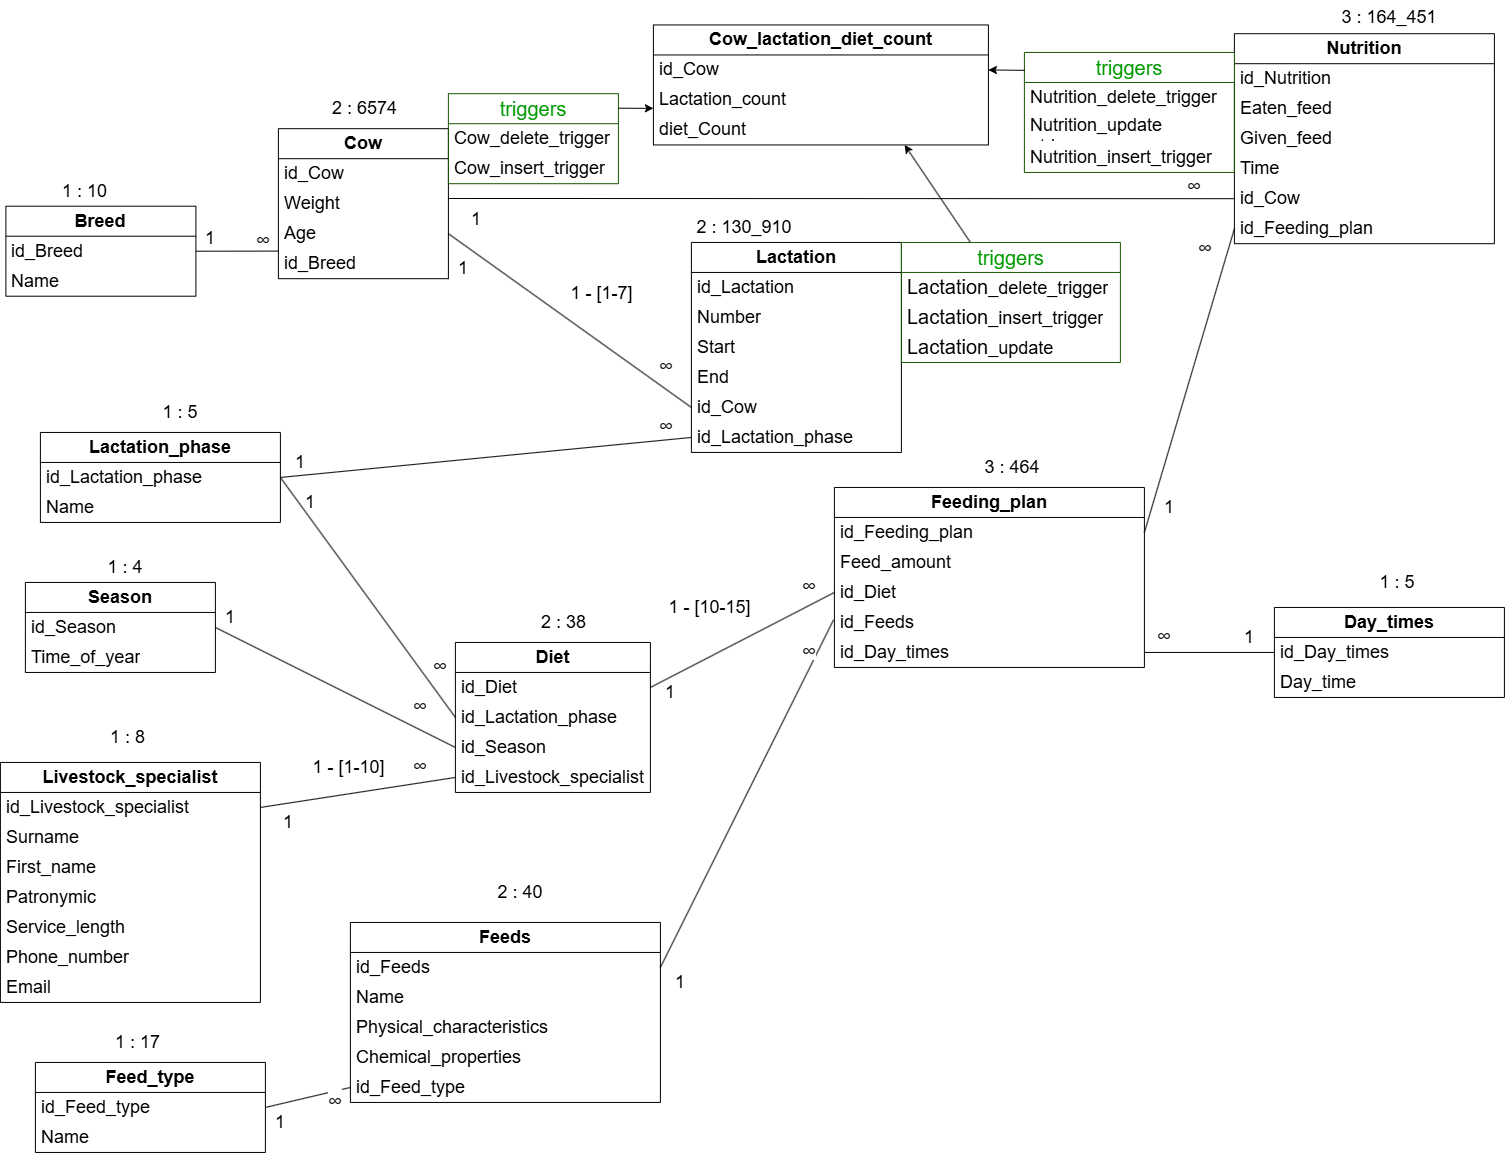
\includegraphics[width=\textwidth, height=\textheight, keepaspectratio]{images/схема_бд_англ_триггеры.png}
        \caption{Схема базы данных на английском языке с триггерами}
        \label{fig:схема_бд_англ}
    \end{figure}
\end{landscape}
\restoregeometry
\clearpage


\subsection{Создание триггеров}

В листинге \ref{lst:Cow_insert_trigger}
приведена SQL-команда создания триггера, срабатывающего после добавления новой записи в таблицу \texttt{Cow}.

\begin{lstlisting}[caption={Создание триггера Cow\_insert\_trigger}, label={lst:Cow_insert_trigger}]
CREATE TRIGGER Cow_insert_trigger
    AFTER INSERT ON Cow 
    FOR EACH ROW EXECUTE FUNCTION Cow_insert_trigger_function();
\end{lstlisting}

В листинге \ref{lst:Cow_insert_trigger_function} представлена SQL-команда создания функции \\
\texttt{Cow\_insert\_trigger\_function}. Функция вызывается триггером \\\texttt{Cow\_insert\_trigger}
и добавляет в таблицу \texttt{Cow\_lactation\_diet\_count} новую запись для зарегистрированной коровы,
инициализируя начальные значения количества лактаций и рационов нулями.
\begin{lstlisting}[caption={Создание функции Cow\_insert\_trigger\_function}, label={lst:Cow_insert_trigger_function}]
CREATE OR REPLACE FUNCTION Cow_insert_trigger_function()
RETURNS TRIGGER AS $$
BEGIN
    INSERT INTO Cow_lactation_diet_count (id_Cow, Lactation_count, Diet_count)
    VALUES (NEW.id_Cow, 0, 0);
    RETURN NEW;
END;
$$ LANGUAGE plpgsql;
\end{lstlisting}

В листинге \ref{lst:Cow_delete_trigger} представлена SQL-команда создания триггера,
срабатывающего после удаления записи из таблицы \texttt{Cow}.

\begin{lstlisting}[caption={Создание триггера Cow\_delete\_trigger}, label={lst:Cow_delete_trigger}]
CREATE TRIGGER Cow_delete_trigger 
    AFTER DELETE ON Cow 
    FOR EACH ROW EXECUTE FUNCTION Cow_delete_trigger_function();
\end{lstlisting}

В листинге \ref{lst:Cow_delete_trigger_function} приведена SQL-команда создания функции \\
\texttt{Cow\_delete\_trigger\_function}.
Функция вызывается триггером \\\texttt{Cow\_delete\_trigger}
и удаляет соответствующую запись из таблицы \texttt{Cow\_lactation\_diet\_count}
по идентификатору удаляемой коровы \\(\texttt{OLD.id\_Cow}).

\begin{lstlisting}[caption={Создание функции Cow\_delete\_trigger\_function}, label={lst:Cow_delete_trigger_function}]
CREATE OR REPLACE FUNCTION Cow_delete_trigger_function()
RETURNS TRIGGER AS $$
BEGIN
    DELETE FROM Cow_lactation_diet_count WHERE id_Cow = OLD.id_Cow;
    RETURN OLD;
END;
$$ LANGUAGE plpgsql;
\end{lstlisting}

В листинге \ref{lst:Nutrition_insert_trigger} представлена SQL-команда создания триггера,
срабатывающего после добавления новой записи в таблицу \texttt{Nutrition}.

\begin{lstlisting}[caption={Создание триггера Nutrition\_insert\_trigger}, label={lst:Nutrition_insert_trigger}]
CREATE TRIGGER Nutrition_insert_trigger
    AFTER INSERT ON Nutrition 
    FOR EACH ROW EXECUTE FUNCTION Nutrition_insert_trigger_function();
\end{lstlisting}

В листинге \ref{lst:Nutrition_insert_trigger_function} приведена SQL-команда создания функции \\
\texttt{Nutrition\_insert\_trigger\_function}.
Функция вызывается триггером \texttt{Nutrition\_insert\_trigger} и выполняет перерасчет количества
уникальных рационов для коровы \texttt{NEW.id\_Cow} (обращение к значению поля id\_Cow из строки,
которая добавлена в таблицу \texttt{Nutrition}) путем объединения таблиц
\texttt{Nutrition, Feeding\_plan} и \texttt{Diet} с помощью \texttt{LEFT JOIN}.
В результате работы функции обновляется значение поля
\texttt{diet\_count} в таблице \texttt{Cow\_lactation\_diet\_count}.

\begin{lstlisting}[caption={Создание функции Nutrition\_insert\_trigger\_function}, label={lst:Nutrition_insert_trigger_function}]
CREATE OR REPLACE FUNCTION Nutrition_insert_trigger_function()
RETURNS TRIGGER AS $$
BEGIN 
    UPDATE Cow_lactation_diet_count 
    SET diet_count = (
        SELECT COUNT(DISTINCT Diet.id_Diet)
        FROM Nutrition
        LEFT JOIN Feeding_plan ON Feeding_plan.id_Feeding_plan = Nutrition.id_Feeding_plan
        LEFT JOIN Diet ON Diet.id_Diet = Feeding_plan.id_Diet
        WHERE Nutrition.id_Cow = NEW.id_Cow
    )
    WHERE id_Cow = NEW.id_Cow; 
    RETURN NEW;
END;
$$ LANGUAGE plpgsql;
\end{lstlisting}

В листинге \ref{lst:Nutrition_delete_trigger} представлена SQL-команда создания триггера,
срабатывающего после удаления записи из таблицы \texttt{Nutrition}.

\begin{lstlisting}[caption={Создание триггера Nutrition\_delete\_trigger}, label={lst:Nutrition_delete_trigger}]
CREATE TRIGGER Nutrition_delete_trigger
    AFTER DELETE ON Nutrition
    FOR EACH ROW EXECUTE FUNCTION Nutrition_delete_trigger_function();
\end{lstlisting}

В листинге \ref{lst:Nutrition_delete_trigger_function} приведена SQL-команда создания функции
\\\texttt{Nutrition\_delete\_trigger\_function}.
Функция вызывается триггером \texttt{Nutrition\_delete\_trigger} и выполняет перерасчет количества
уникальных рационов для коровы \texttt{OLD.id\_Cow} (обращение к значению поля id\_Cow из строки,
которая удалена из таблицы \texttt{Nutrition}) после удаления соответствующей записи.
Результат повторного вычисления обновляет значение столбца \texttt{diet\_count} в таблице
\texttt{Cow\_lactation\_diet\_count}.

\begin{lstlisting}[caption={Создание функции Nutrition\_delete\_trigger\_function}, label={lst:Nutrition_delete_trigger_function}]
CREATE OR REPLACE FUNCTION Nutrition_delete_trigger_function()
RETURNS TRIGGER AS $$
BEGIN
    UPDATE Cow_lactation_diet_count 
    SET diet_count = (
        SELECT COUNT(DISTINCT Diet.id_Diet)
        FROM Nutrition
        LEFT JOIN Feeding_plan ON Feeding_plan.id_Feeding_plan = Nutrition.id_Feeding_plan
        LEFT JOIN Diet ON Diet.id_Diet = Feeding_plan.id_Diet
        WHERE Nutrition.id_Cow = OLD.id_Cow
    )
    WHERE id_Cow = OLD.id_Cow; 
    RETURN OLD;
END;
$$ LANGUAGE plpgsql;
\end{lstlisting}

В листинге \ref{lst:Nutrition_update_trigger} представлена SQL-команда создания триггера,
срабатывающего после обновления записи в таблице \texttt{Nutrition}.
Данная реализация рассчитана на случай изменения только плана кормления.

\begin{lstlisting}[caption={Создание триггера Nutrition\_update\_trigger}, label={lst:Nutrition_update_trigger}]
CREATE TRIGGER Nutrition_update_trigger
    AFTER UPDATE ON Nutrition 
    FOR EACH ROW EXECUTE FUNCTION Nutrition_update_trigger_function();
\end{lstlisting}

В листинге \ref{lst:Nutrition_update_trigger_function} приведена SQL-команда создания функции
\\\texttt{Nutrition\_update\_trigger\_function}.
Функция вызывается триггером \texttt{Nutrition\_update\_trigger} после изменения записи
в таблице \texttt{Nutrition} и выполняет перерасчет количества уникальных рационов для коровы
\texttt{NEW.id\_Cow}, заменяя устаревшее значение в столбце \texttt{diet\_count}
таблицы \texttt{Cow\_lactation\_diet\_count} на актуальное.

\begin{lstlisting}[caption={Создание функции Nutrition\_update\_trigger\_function}, label={lst:Nutrition_update_trigger_function}]
CREATE OR REPLACE FUNCTION Nutrition_update_trigger_function()
RETURNS TRIGGER AS $$
BEGIN
    UPDATE Cow_lactation_diet_count 
    SET diet_count = (
        SELECT COUNT(DISTINCT Diet.id_Diet)
        FROM Nutrition
        LEFT JOIN Feeding_plan ON Feeding_plan.id_Feeding_plan = Nutrition.id_Feeding_plan
        LEFT JOIN Diet ON Diet.id_Diet = Feeding_plan.id_Diet
        WHERE Nutrition.id_Cow = NEW.id_Cow
    )
    WHERE id_Cow = NEW.id_Cow;
    RETURN NEW; 
END;
$$ LANGUAGE plpgsql;
\end{lstlisting}

В листинге \ref{lst:Lactation_insert_trigger} представлена SQL-команда создания триггера,
срабатывающего после добавления новой записи в таблицу \texttt{Lactation}.

\begin{lstlisting}[caption={Создание триггера Lactation\_insert\_trigger}, label={lst:Lactation_insert_trigger}]
CREATE TRIGGER Lactation_insert_trigger
    AFTER INSERT ON Lactation 
    FOR EACH ROW EXECUTE FUNCTION Lactation_insert_trigger_function();
\end{lstlisting}

В листинге \ref{lst:Lactation_insert_trigger_function} приведена SQL-команда создания функции
\\\texttt{Lactation\_insert\_trigger\_function}.
Функция вызывается триггером \texttt{Lactation\_insert\_trigger} при добавлении нового периода лактации
и выполняет перерасчет общего количества лактаций для соответствующей коровы \texttt{NEW.id\_Cow},
обновляя значение столбца \texttt{lactation\_count} в таблице \texttt{Cow\_lactation\_diet\_count}.

\begin{lstlisting}[caption={Создание функции Lactation\_insert\_trigger\_function}, label={lst:Lactation_insert_trigger_function}]
CREATE OR REPLACE FUNCTION Lactation_insert_trigger_function()
RETURNS TRIGGER AS $$
BEGIN
    UPDATE Cow_lactation_diet_count 
    SET lactation_count = 
        (SELECT COUNT(*) FROM Lactation WHERE id_Cow = NEW.id_Cow)
    WHERE id_Cow = NEW.id_Cow;
    RETURN NEW;
END;
$$ LANGUAGE plpgsql;
\end{lstlisting}


В листинге \ref{lst:Lactation_delete_trigger} представлена SQL-команда создания триггера,
срабатывающего после удаления записи из таблицы \texttt{Lactation}.

\begin{lstlisting}[caption={Создание триггера Lactation\_delete\_trigger}, label={lst:Lactation_delete_trigger}]
CREATE TRIGGER Lactation_delete_trigger
    AFTER DELETE ON Lactation
    FOR EACH ROW EXECUTE FUNCTION Lactation_delete_trigger_function();
\end{lstlisting}

В листинге \ref{lst:Lactation_delete_trigger_function} приведена SQL-команда создания функции
\\\texttt{Lactation\_delete\_trigger\_function}.
Функция вызывается триггером \texttt{Lactation\_delete\_trigger} и выполняет
перерасчет количества лактаций для соответствующей коровы \texttt{OLD.id\_Cow},
обновляя значение столбца \texttt{lactation\_count} таблицы \texttt{Cow\_lactation\_diet\_count}.

\begin{lstlisting}[caption={Создание функции Lactation\_delete\_trigger\_function}, label={lst:Lactation_delete_trigger_function}]
CREATE OR REPLACE FUNCTION Lactation_delete_trigger_function()
RETURNS TRIGGER AS $$
BEGIN
    UPDATE Cow_lactation_diet_count 
    SET lactation_count = 
        (SELECT COUNT(*) FROM Lactation WHERE id_Cow = OLD.id_Cow)
    WHERE id_Cow = OLD.id_Cow;  
    RETURN OLD;
END;
$$ LANGUAGE plpgsql;
\end{lstlisting}

В листинге \ref{lst:Lactation_update_trigger} представлена SQL-команда создания триггера,
срабатывающего после обновления записи в таблице \texttt{Lactation}.
Данная реализация не рассчитана на случай изменения \texttt{id\_Cow} коровы.

\begin{lstlisting}[caption={Создание триггера Lactation\_update\_trigger}, label={lst:Lactation_update_trigger}]
CREATE TRIGGER Lactation_update_trigger
    AFTER UPDATE ON Lactation 
    FOR EACH ROW EXECUTE FUNCTION Lactation_update_trigger_function();
\end{lstlisting}

В листинге \ref{lst:Lactation_update_trigger_function} приведена SQL-команда создания функции
\\\texttt{Lactation\_update\_trigger\_function}.
Функция вызывается триггером \texttt{Lactation\_update\_trigger}
и выполняет перерасчет количества лактаций для соответствующей коровы \texttt{NEW.id\_Cow},
обновляя значение столбца \texttt{lactation\_count} в таблице \texttt{Cow\_lactation\_diet\_count}.

\begin{lstlisting}[caption={Создание функции Lactation\_update\_trigger\_function}, label={lst:Lactation_update_trigger_function}]
CREATE OR REPLACE FUNCTION Lactation_update_trigger_function()
RETURNS TRIGGER AS $$
BEGIN
    UPDATE Cow_lactation_diet_count
    SET lactation_count =
        (SELECT COUNT(*) FROM Lactation WHERE id_Cow = NEW.id_Cow)
    WHERE id_Cow = NEW.id_Cow;
    RETURN NEW;
END;
$$ LANGUAGE plpgsql;
\end{lstlisting}

\subsection{Демонстрация работы триггеров}

В таблице \ref{tab:действия_триггеров} представлено описание изменений 
таблицы \\\texttt{Cow\_lactation\_diet\_count} 
посредством триггеров в зависимости от изменения данных в таблицах \texttt{Cow},
\texttt{Nutrition}, \texttt{Lactation}.

\begin{table}[h!]
\centering
\caption{Описание действий триггеров}
\label{tab:действия_триггеров}
\begin{tabular}{|c|p{0.85\textwidth}|}
\hline
\textnumero & {Действие} \\
\hline
1 & Добавление коровы в таблицу \texttt{Cow}. В таблице \texttt{Cow\_lactation\_diet\_count} создаётся запись с нулевыми значениями количества лактаций и рационов. \\
\hline
2 & Удаление коровы из таблицы \texttt{Cow}. Из таблицы \texttt{Cow\_lactation\_diet\_count} удаляется соответствующая запись. \\
\hline
3 & Добавление записи питания в таблицу \texttt{Nutrition}. Пересчитывается количество уникальных рационов для указанной коровы в таблице \texttt{Cow\_lactation\_diet\_count}. \\
\hline
4 & Удаление записи питания из таблицы \texttt{Nutrition}. Пересчитывается количество уникальных рационов для указанной коровы в таблице \texttt{Cow\_lactation\_diet\_count}. \\
\hline
5 & Изменение плана кормления в таблице \texttt{Nutrition}. Пересчитывается количество уникальных рационов для указанной коровы в таблице \texttt{Cow\_lactation\_diet\_count}. \\
\hline
6 & Добавление лактации в таблицу \texttt{Lactation}. Пересчитывается общее количество лактаций для указанной коровы в таблице \texttt{Cow\_lactation\_diet\_count}. \\
\hline
7 & Удаление лактации из таблицы \texttt{Lactation}. Пересчитывается общее количество лактаций для указанной коровы в таблице \texttt{Cow\_lactation\_diet\_count}. \\
\hline
\end{tabular}
\end{table}

На рисунке \ref{cow_insert_example} представлено появление новой записи
в таблице \\\texttt{Cow\_lactation\_diet\_count} после добавления
записи в таблицу \texttt{Cow}.

\begin{figure}[H]
    \centering
    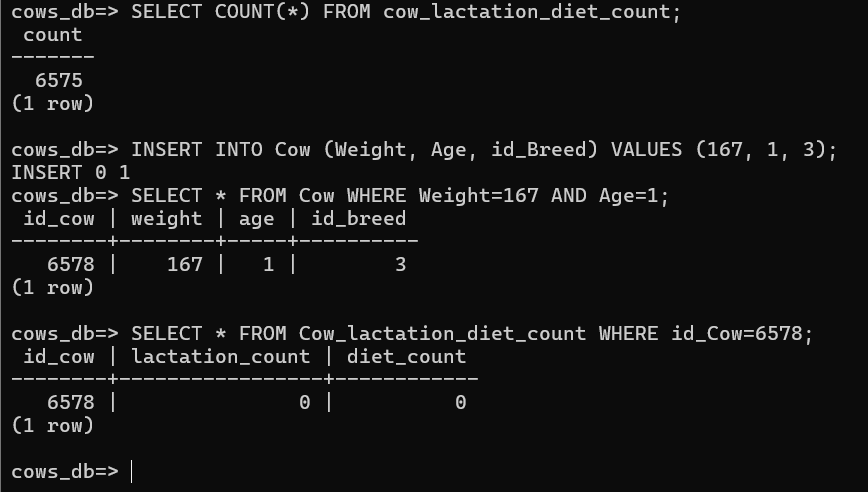
\includegraphics[width=\linewidth]{images/cow_insert_example.png}
    \caption{Результат добавления новой записи в таблицу Cow}
    \label{cow_insert_example}
\end{figure}

На рисунке \ref{delete_cow_example} представлены изменения данных в таблице \\
\texttt{Cow\_lactation\_diet\_count}: отсутствие данных о корове, запись которой
была удалена из таблицы \texttt{Cow}.

\begin{figure}[H]
    \centering
    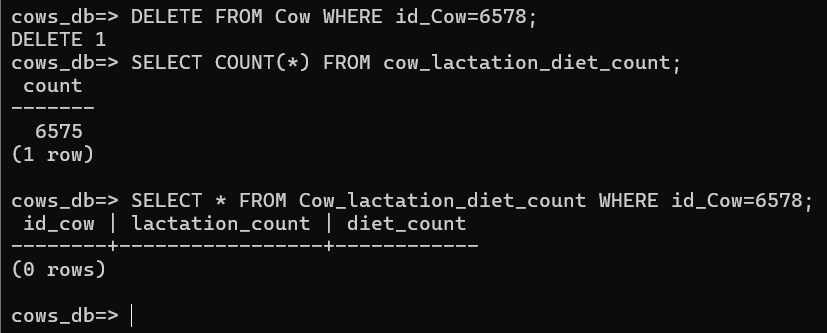
\includegraphics[width=\linewidth]{images/delete_cow_example.png}
    \caption{Результат удаления записи из таблицы Cow}
    \label{delete_cow_example}
\end{figure}

На рисунке \ref{delete_lactation_example} продемонстрировано уменьшение
количества лактаций в таблице
{Cow\_lactation\_diet\_count} после удаления записи в таблице
\texttt{Lactation}.

\begin{figure}[H]
    \centering
    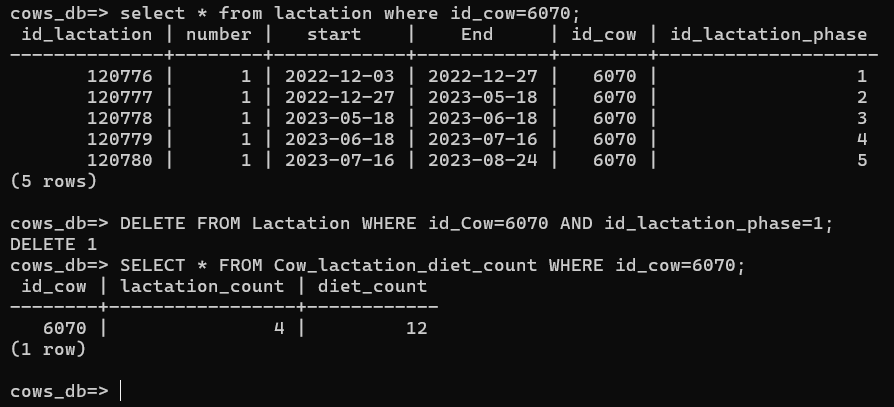
\includegraphics[width=\linewidth]{images/delete_lactation_example.png}
    \caption{Результат удаления записи из таблицы Lactation}
    \label{delete_lactation_example}
\end{figure}

На рисунке \ref{update_nutrition_example} продемонстрировано уменьшение количества
рационов в таблице
\texttt{Cow\_lactation\_diet\_count} после изменения плана кормления
в таблице \texttt{Nutrition}.

\begin{figure}[H]
    \centering
    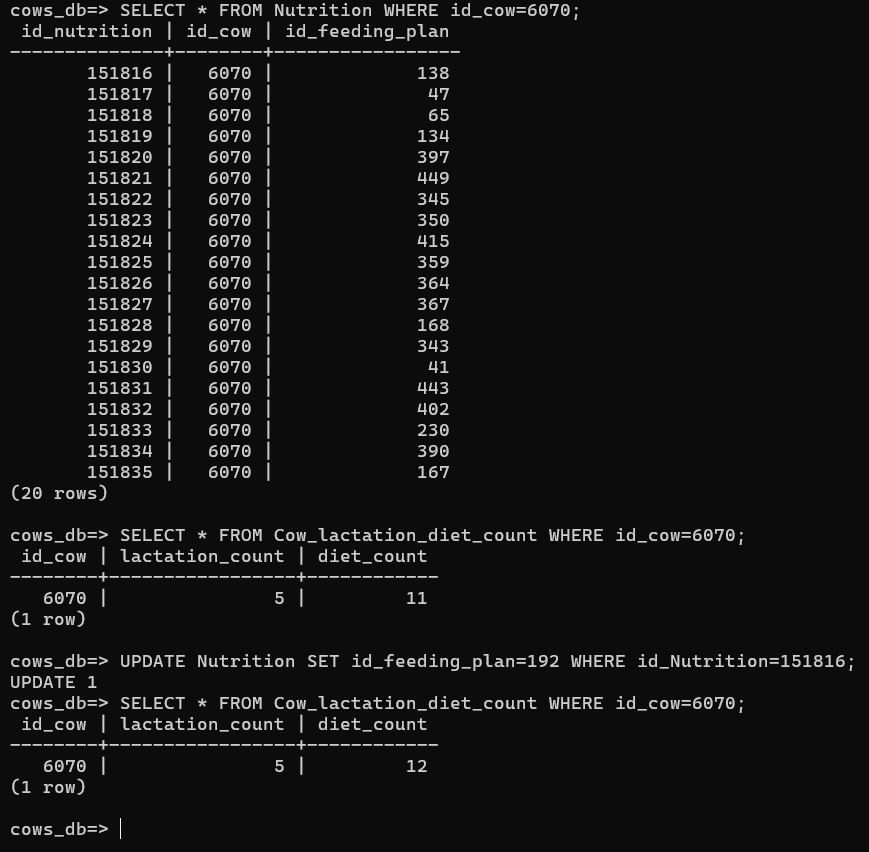
\includegraphics[width=\linewidth]{images/update_nutrition_example.png}
    \caption{Изменение данных при обновлении плана кормления в таблице Nutrition}
    \label{update_nutrition_example}
\end{figure}


\newpage

\addcontentsline{toc}{section}{Заключение раздела <<Триггеры>>}
\section*{Заключение раздела <<Триггеры>>}

В результате работы была создана таблица \texttt{Cow\_lactation\_diet\_count}
и заполнена данными на основе агрегатных вычислений по таблицам
\texttt{Cow}, \texttt{Lactation}, \texttt{Nutrition}, \texttt{Feeding\_plan}
и \texttt{Diet}. Для автоматического поддержания актуальности данных
созданы 7 триггеров: для таблицы \texttt{Cow} --- при добавлении
и удалении записей; для таблицы \texttt{Nutrition} --- при добавлении,
удалении и изменении плана кормления; для таблицы \texttt{Lactation} ---
при добавлении и удалении периодов лактации.
\newpage



\section{Права доступа}
\textbf{Формулировка задания.}
Создать двух пользователей с следующими правами:
один из пользователей должен иметь право только на просмотр таблицы
\texttt{Cow\_lactation\_diet\_count}, а второй пользователь ---
на просмотр и изменение
таблиц \texttt{Cow}, \texttt{Lactation}, \texttt{Nutrition}.

\subsection{Создание пользователей}

В ходе работы были созданы два пользователя: resultsReader,\\
resultsEditor
(см. листинг \ref{lst:создание_пользователей}).

\begin{lstlisting}[caption={Создание пользователей}, label={lst:создание_пользователей}]
CREATE USER resultsReader WITH PASSWORD '*';
CREATE USER resultsEditor WITH PASSWORD '*';
\end{lstlisting}

В листинге \ref{lst:права_на_бд} представлены SQL-команды,
которые обеспечивают доступ новым пользователям к объектам базы данных.
Первая команда предоставляет обоим пользователям право подключения
к базе данных \texttt{cows\_db}.
Вторая команда предоставляет возможность обоим пользователям
обращаться к объектам, расположенным в схеме public.
Третья команда выдаёт пользователю \texttt{resultsEditor} право на
использование всех последовательностей в схеме public,
что необходимо для создания новых записей в таблицах,
содержащих автоинкрементные поля (SERIAL).

\begin{lstlisting}[caption={Общие права на базу данных}, label={lst:права_на_бд}]
GRANT CONNECT ON DATABASE cows_db TO resultsReader, resultsEditor;
GRANT USAGE ON SCHEMA public TO resultsReader, resultsEditor;
GRANT USAGE ON ALL SEQUENCES IN SCHEMA public TO resultsEditor;
\end{lstlisting}

В листинге \ref{lst:права_на_таблицы} представлены SQL-команды,
с помощью которых новым пользователям были выданы права на чтение или изменение
таблиц. Пользователю resultsReader выдано право только на чтение таблицы
\texttt{Cow\_lactation\_diet\_count}, а пользователю \texttt{resultsEditor} ---
на чтение и изменение таблиц \texttt{Cow}, \texttt{Lactation}, \texttt{Nutrition}.

\begin{lstlisting}[caption={Права на таблицы}, label={lst:права_на_таблицы}]
GRANT SELECT ON Cow_lactation_diet_count TO resultsReader;
GRANT SELECT, INSERT, DELETE, UPDATE ON Cow, Lactation, Nutrition TO resultsEditor;
\end{lstlisting}

В листинге \ref{lst:изм_триг_функ} представлено изменение
триггерных функций. Добавлено \texttt{SECURITY DEFINER}~---
выполнение функции с правами её создателя, а не вызывающего.
Это необходимо для того, чтобы при изменении таблиц пользователем
\texttt{resultsEditor} вызывались триггерные функции,
несмотря на то что текущий пользователь не имеет доступа к таблице\\
\texttt{Cow\_lactation\_diet\_count}, обновляемой триггерами.

\begin{lstlisting}[caption={Изменение триггерных функций}, label={lst:изм_триг_функ}]
ALTER FUNCTION Cow_insert_trigger_function() SECURITY DEFINER;
ALTER FUNCTION Cow_delete_trigger_function() SECURITY DEFINER;
ALTER FUNCTION Nutrition_insert_trigger_function() SECURITY DEFINER;
ALTER FUNCTION Nutrition_delete_trigger_function() SECURITY DEFINER;
ALTER FUNCTION Nutrition_update_trigger_function() SECURITY DEFINER;
ALTER FUNCTION Lactation_insert_trigger_function() SECURITY DEFINER;
ALTER FUNCTION Lactation_delete_trigger_function() SECURITY DEFINER;
ALTER FUNCTION Lactation_update_trigger_function() SECURITY DEFINER;
\end{lstlisting}

\subsection{Результаты работы}

На рисунке \ref{select_editor_err} представлен вывод ошибки при попытке
просмотра таблицы \texttt{Cow\_lactation\_diet\_count} пользователем
\texttt{resultsEditor}.
\begin{figure}[H]
    \centering
    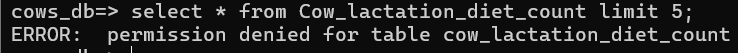
\includegraphics[width=\linewidth]{images/select_editor_err.png}
    \caption{Ошибка доступа пользователя \texttt{resultsEditor} к таблице \texttt{Cow\_lactation\_diet\_count}}
    \label{select_editor_err}
\end{figure}

На рисунке \ref{select_editor_ok} представлен вывод строк из таблиц
\texttt{Cow}, \texttt{Lactation}, \texttt{Nutrition} после запросов
\texttt{SELECT} пользователем \texttt{resultsEditor}.
\begin{figure}[H]
    \centering
    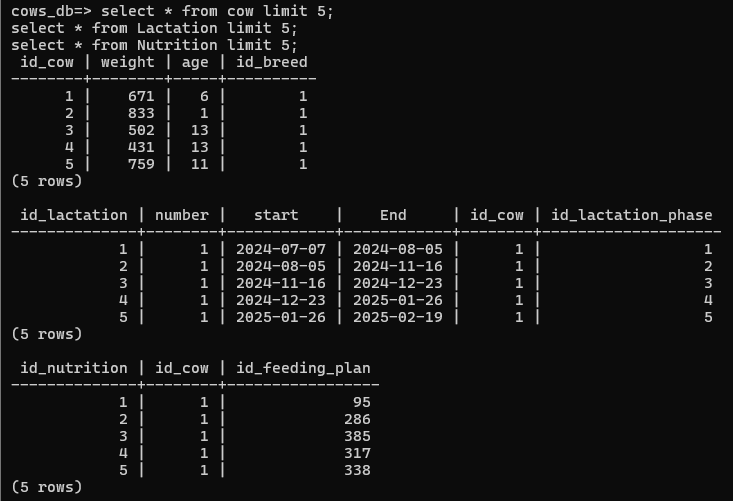
\includegraphics[width=\linewidth]{images/select_editor_ok.png}
    \caption{Успешный просмотр таблиц \texttt{Cow}, \texttt{Lactation}, \texttt{Nutrition} пользователем \texttt{resultsEditor}}
    \label{select_editor_ok}
\end{figure}

На рисунке \ref{select_reader_ok} представлен вывод строк из таблицы
\texttt{Cow\_lactation\_diet\_count} после запроса \texttt{SELECT}
пользователем \texttt{resultsReader}.
\begin{figure}[H]
    \centering
    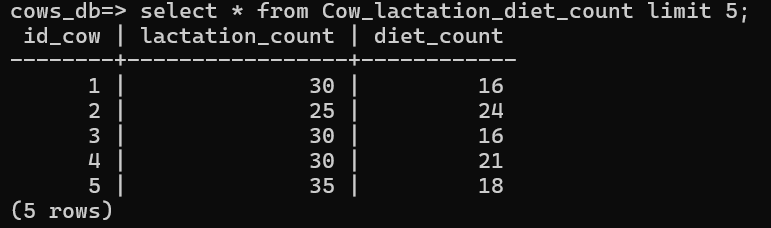
\includegraphics[width=0.8\linewidth]{images/select_reader_ok.png}
    \caption{Успешный просмотр таблицы \texttt{Cow\_lactation\_diet\_count} пользователем \texttt{resultsReader}}
    \label{select_reader_ok}
\end{figure}

На рисунке \ref{select_reader_err} представлен вывод ошибки при
попытке просмотра таблицы \texttt{Cow}
пользователем \texttt{resultsReader}.
\begin{figure}[H]
    \centering
    
\includegraphics[width=0.7\linewidth]{images/select_reader_err.png}
    \caption{Ошибка доступа пользователя \texttt{resultsReader} к таблице \texttt{Cow}}
    \label{select_reader_err}
\end{figure}

На рисунке \ref{edit_cow} представлен пример добавления записи в таблицу
\texttt{Cow} пользователем \texttt{resultsEditor}, а также изменение и удаление
этой записи.
\begin{figure}[H]
    \centering
    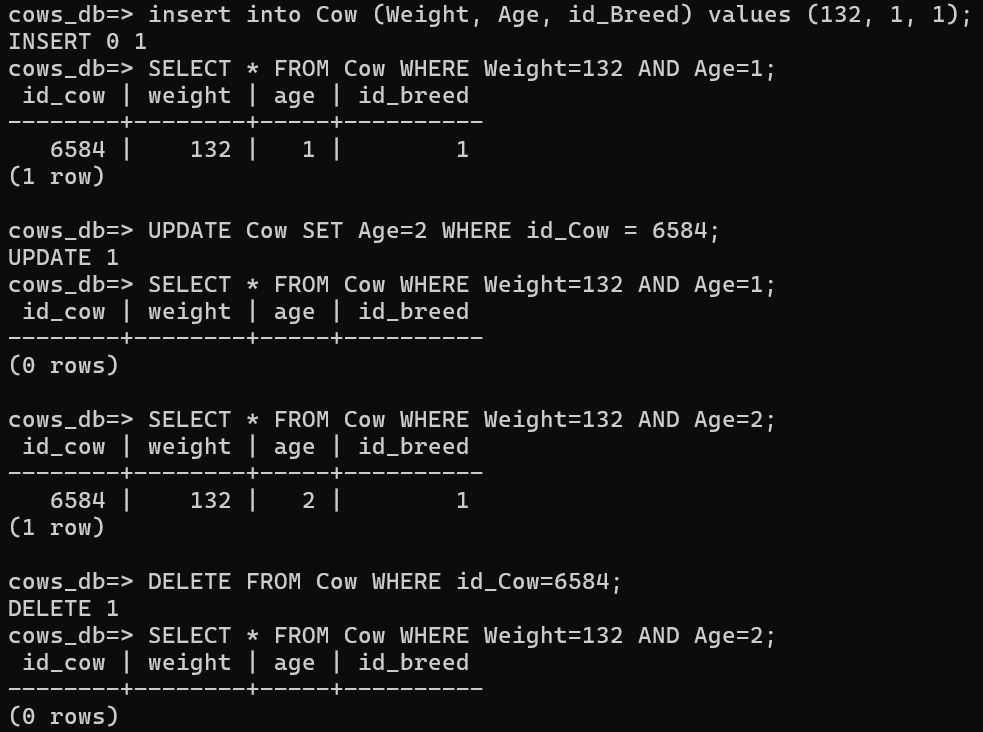
\includegraphics[width=0.9\linewidth]{images/edit_cow.png}
    \caption{Операции \texttt{INSERT}, \texttt{UPDATE} и \texttt{DELETE} в таблице \texttt{Cow} пользователем \texttt{resultsEditor}}
    \label{edit_cow}
\end{figure}

На рисунке \ref{after_insert} представлен пример добавления записи
в таблицу \texttt{Cow} пользователем \texttt{resultsEditor}
и автоматическое добавление записи в таблицу \texttt{Cow\_lactation\_diet\_count}.
\begin{figure}[H]
    \centering
    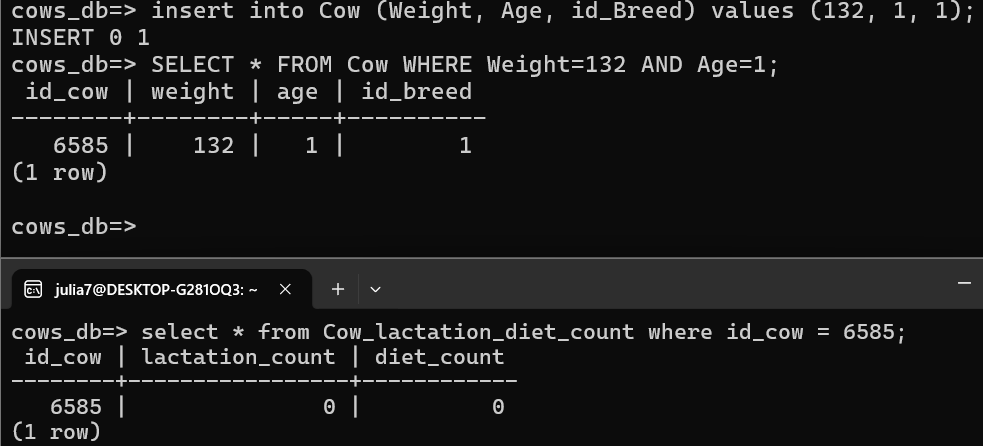
\includegraphics[width=0.9\linewidth]{images/after_insert.png}
    \caption{Автоматическое обновление таблицы триггером при добавлении записи в таблицу \texttt{Cow}}
    \label{after_insert}
\end{figure}

В таблице \ref{tab:проверка_прав} приведены сравнительные результаты
проверки прав доступа пользователей.

\begin{table}[h!]
\centering
\caption{Результаты проверки прав доступа пользователей}
\label{tab:проверка_прав}
\begin{tabular}{|c|c|c|}
\hline
\textnumero & \textbf{resultsReader} & \textbf{resultsEditor} \\
\hline
\multicolumn{3}{|c|}{\texttt{SELECT * FROM Cow\_lactation\_diet\_count LIMIT 5;}} \\
\hline
1 & Результат запроса & Ошибка доступа \\
\hline
\multicolumn{3}{|c|}{\texttt{SELECT * FROM Cow LIMIT 5;}} \\
\hline
2 & Ошибка доступа & Результат запроса \\
\hline
\multicolumn{3}{|c|}{\texttt{INSERT INTO Cow (Weight, Age, id\_Breed) VALUES (160, 2, 3);}} \\
\hline
3 & Ошибка доступа & Выполненный запрос \\
\hline
\multicolumn{3}{|c|}{\texttt{UPDATE Cow SET Age = 2 WHERE id\_Cow = 6584;}} \\
\hline
4 & Ошибка доступа & Выполненный запрос \\
\hline
\multicolumn{3}{|c|}{\texttt{DELETE FROM Cow WHERE id\_Cow = 6584;}} \\
\hline
5 & Ошибка доступа & Выполненный запрос \\
\hline
\multicolumn{3}{|c|}{\texttt{SELECT * FROM Lactation LIMIT 5;}} \\
\hline
6 & Ошибка доступа & Результат запроса \\
\hline
\multicolumn{3}{|c|}{\texttt{SELECT * FROM Breed LIMIT 5;}} \\
\hline
7 & Ошибка доступа & Ошибка доступа \\
\hline
\end{tabular}
\end{table}
\newpage


\addcontentsline{toc}{section}{Заключение раздела <<Права доступа>>}
\section*{Заключение раздела <<Права доступа>>}

В результате выполнения работы были созданы две учётные записи пользователей.
Были выданы базовые права на подключение к базе данных и использование схемы,
а также права на использование последовательностей для пользователя \texttt{resultsEditor}.
Затем были выданы права на таблицы: пользователю \texttt{resultsReader} ---
на чтение таблицы \texttt{Cow\_lactation\_diet\_count},
а пользователю \texttt{resultsEditor} --- на чтение и изменение таблиц
\texttt{Cow}, \texttt{Lactation}, \texttt{Nutrition}.
Для корректной работы триггеров при операциях от имени \texttt{resultsEditor}
все триггерные функции были переведены в режим \texttt{SECURITY DEFINER}.
\newpage




\addcontentsline{toc}{section}{Список литературы}
\begin{thebibliography}{99}

\bibitem{косарева2020}
Косарева Н.А., Чаунина Е.А., Ахмиева Г.Р., Петрова М.Ю. 
Влияние качества кормовых рационов на производство молока // 
Современное состояние, перспективы развития АПК и производства специализированных продуктов питания: 
материалы Международной научно-практической конференции, посвящённой юбилею Заслуженного работника 
высшей школы Российской Федерации, доктора технических наук, профессора Гавриловой Натальи Борисовны, 
24 апреля 2020 года. – Омск: Омский ГАУ, 2020. – С. 700–706.

\end{thebibliography}




\end{document}
% !TEX root = main.tex